\chapter{Flash-Speicher\label{chapter:flash}}
\lhead{Flash-Speicher}
\begin{refsection}
\chapterauthor{Roger Billeter und Gabriel Looser}

\begin{figure}
\centering
\includegraphics{flash/potential-1.pdf}
\caption{St"orpotential f"ur das Modell f"ur den Schreibprozess bei
einem Flashspeicher}
\end{figure}

\section{Einleitung}
\rhead{Einleitung}
Der Flash-Speicher ist ein elektrisches Speicherelement, welches
weit verbreitet ist. Grunds"atzlich wird zwischen zwei Vorg"angen
unterschieden, dem Schreib- und dem L"oschvorgang. Der L"oschvorgang
beruht auf dem Tunneleffekt, welcher im Kapitel Tunneldiode ausf"uhrlich
erkl"art wird. F"ur den Speichervorgang m"ussen Elektronen mittels
'hot electron injection' in das Floating-Gate gebracht werden.

\section{Flash-Typen}
\rhead{Flash-Typen}
Bei den Flash-Speichern wird zwischen zwei Typen unterschieden, den NAND
und den NOR Typen. Diese unterscheiden sich in der Zusammenschaltung
der einzelnen Transistoren.

\subsection{NAND Typ}
\rhead{NAND Typ}
Bei den NAND Flash-Speicher werden die einzelnen Transistoren zu einer
NAND Speicherzelle zusammen geschaltet. Die Speicherzellen werden in
Gruppen in Serie geschaltet. Die Speicherzellengruppe teilt sich eine
Datenleitung, daher muss das Lesen und Schreiben immer in der ganzen
Gruppe sequentiell erfolgen. Dadurch wird die Anzahl Datenleitungen
reduziert und der Flash-Speicher ben"otigt weniger Platz. NAND
Flash-Speicher haben ihre Verwendung vor allem in Bereichen, wo viel
Speicher m"oglichst wenig Platz brauchen darf und die Zugriffszeit keine
grosse Rolle spielt.
\subsection{NOR Typ}
\rhead{NOR Typ}
Bei den NOR Flash-Speicher werden die Transistoren zu einer NOR
Speicherzelle zusammen geschaltet.
Die Speicherzellen werden "uber die Datenleitungen parallel geschaltet,
dadurch kann auf jede Speicherzelle direkt zugegriffen werden. Die
Parallelleitungen brauchen mehr Platz, es lassen sich jedoch k"urzere
Zugriffszeiten realisieren.

\section{Floating Gate Transistor}
\rhead{Floating Gate}
Floating Gate Transistoren z"ahlen zu den Feldeffekttransistoren
(Siehe Abbildung \ref{skript:Floatinggatetransistor}). Die Absicht ist
es den Zustand des Floating Gates zu erh"ohen. Dies kann man erreichen,
indem im Floating Gate eine gewisse Ladung gespeichert wird. Diese kann
erh"oht werden, indem das Potential am Control Gate erh"oht wird. Nun
fliessen die Elektronen in Richtung Source.

\begin{figure}
\centering
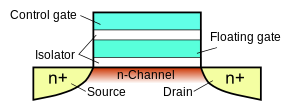
\includegraphics[width=0.7\textwidth]{flash/graphics/Floatinggate.png}
\caption{Abbildung eines Floating Gate Transistors: Quelle:
\url{http://upload.wikimedia.org/wikipedia/commons/a/ae/Floating_gate_transistor-en.svg}
\label{skript:Floatinggatetransistor}}
\end{figure}

Je nachdem was es f"ur ein Potential am Control Gate hat, k"onnen mehrere
Zust"ande gespeichert werden. In einem Floating Gate Transistor kann
man auch mehrere Bits speichern, "ublicherweise werden 2 Bits gespeichert.
Der Source Anschluss wird meistens mit GND verbunden und Drain wird beim
Leseprozess auf 0V gehängt und beim Schreibeprozess "ublicherweise auf
"uber 10V.


\section{Zyklenzahlen}
\rhead{Zyklenzahlen}
Ein grosses Problem bei Flashspeichern ist die begrenzte schreib-und
Leseanzahl. Wegem dem Tunneleffekt fliessen die Elektronen durch die
Oxidschicht, dadurch wird diese Oxidschicht, um das Floating Gate herum,
immer ein kleines bisschen besch"adigt. Dies bewirkt, dass immer mehr
der Ladung abfliessen kann. Bei den NOR-Flashs hat man etwa 10'000
bis 100'000 Zyklen. Hingegen bei den NAND-Flashs sind es doch gegen 2
Millionen Zyklen. Dieses Problem ist jedoch nicht so problematisch, da
der Speicher mit einzelnen Bl"ocken aufgebaut ist. Wenn einer ausf"allt
hat man immer noch einige andere Speicherzellen.


\section{L"oschvorgang}
\rhead{Lo"schvorgang}
Der L"oschvorgang kann erreicht werden, indem das Potential am Gate
heruntergesetzt wird. So wird erreicht, dass es zum Tunneleffekt
kommt. Dies kann im Kapitel \ref{chapter:Tunneleffekt} nachgelesen werden.


\section{Schreibvorgang}

\subsection{Modell des Potentialtopf}
\rhead{Modell des Potentialtopf}
Als Modell f"ur das Floating-Gate wird ein Potentialtopf verwendet,
in dem die Elektronen gespeichert werden.
Als Vereinfachung des Schreibvorgangs kann man sich das Putten beim
Golf vorstellen. Das Elektron ist der Golfball und der Potentialtopf
das Loch. Das Elektron landet jedoch nicht wegen der Schwerkraft im
Potentialtopf, sondern es gibt Energie ab an den Potentialtopf und wird
dadurch abgebremst. Wird das Elektron stark genug abgebremst, landet es
im Potentialtopf.

Am Anfang befindet sich im Potentialtopf ein Grundpotential $E_{0}$
das Ziel ist es dieses Potential auf ein h"oheres Potential $E_{1}$
zu bringen. Da die L"osung der urspr"unglichen Gleichung auf ein
partielles Differential-Gleichungssystem f"uhrt und da das L"osen
partieller Differentialgleichungen nicht Stoff des Bachelorstudiums
ist, werden die Gleichungen mittels Skalarpordukt auf ein normales
Differential-Gleichungssystem vereinfacht. Schlussendlich wird die
Wahrscheinlichkeit eines Zustandes im Potentialtopf errechnet. Diese
Wahrscheinlichkeit ist abh"angig von der Energie des Elektrons, vom
Abstand des Elektrons zum Potentialtopf und der Geschwindigkeit respektive
der Zeit mit der das Elektron auf den Potentialtopf wirkt
%(Bild Potentialtopf).

\subsection{Anregung}
\rhead{Anregung}
Der Potentialtopf mit dem Grundenergie $E_{0}$ hat eine Grundschwingung
$\cos(x)$.  Als Vereinfachung dieser Grundschwingung dient die
Vorstellung eines Wackelpuddings, welcher durch das vorbei fliegende
Elektron zus"atzlich in Schwingung versetzt wird.  Das Grundenergie
wird asymmetrisch angeregt. Wenn man das auf das Modell des
Wackelpudding "ubertr"agt, erkennt man, dass wenn man einen Wackelpudding
gleichm"assig zusammendrückt, wird dieser nicht zus"atzlich in Schwingung
versetzt. Wird der Wackelpudding jedoch auf der einen Seite angestossen,
wird der Wackelpudding zus"atzlich in Schwingung versetzt und erreicht
ein h"oheres Energieniveau.  F"ur die Berechnung wird der Potentialtopf
"uber die h"alfe mit einem Rechteckimpuls angeregt. Dies vereinfacht
das L"osen der Differentialgleichungen.
%(Bild Anregung)

\subsection{Berechnung}
\subsubsection{Schr"odingergleichung}

\rhead{Schr"odingergleichung}
Die Schr"odingergleichung ergibt sich aus der kinetischen Energie des
Potentialtopfes und der potentiellen Energie der Anregung.
\[
\ i\hbar\frac{d}{dt}|\psi(t)\rangle = H|\psi(t)\rangle = (-\frac{\hbar^2}{2m} \frac{\partial^2}{\partial x^2}+V(x)+V_{e}(x,t))|\psi(t)\rangle
\]

Wenn man den Zustand nun von 0 auf 1 erh"oht sieht dies folgendermassen aus:
\[
\ i\hbar\frac{d}{dt}\langle1|\psi(t)\rangle = \langle1|-\frac{\hbar^2}{2m} \frac{\partial^2}{\partial x^2}+V(x)+V_{e}(x,t)|\psi(t)\rangle
\]

Was nun genauer ausgerechnet wird ist $\langle1|\psi(t)\rangle$, denn
dies entspricht der Wahrscheinlichkeit, dass der $|1\rangle$ erreicht ist.

Wenn man die Gleichung nun noch vereinfacht, sieht man, dass diese
Wahrscheinlichkeit mehrfach vorkommt.
\[
\ i\hbar\frac{d}{dt}\langle1|\psi(t)\rangle = E_{1}\langle1|\psi(t)\rangle+\langle1|\psi(t)\rangle V(t)
\]

Das Ganze kann man nun auch mit dem Zustand $|0\rangle$ machen. Diese
Gleichung sieht sehr "ahnlich aus.
\[
\ i\hbar\frac{d}{dt}\langle0|\psi(t)\rangle = E_{0}\langle0|\psi(t)\rangle+\langle0|\psi(t)\rangle V(t)
\]

\subsubsection{Skalarprodukt}
\rhead{Skalarprodukt}
Mittels Skalarprodukt kann das Differentialgleichungssystem weiter
vereinfacht werden.
Denn wie man weiss ergibt das Skalarprodukt von $\langle0|0\rangle$
und $\langle1|1\rangle = 1$. Genauso wie das Skalarprodukt von
$\langle0|1\rangle$ und $\langle1|0\rangle = 0$.
Ausserdem kann  $\langle0|V(t)|0\rangle$ als $V_{0}v_{00}$
geschrieben werden, $\langle1|V(t)|0\rangle$ als
$V_{0}v_{01}$,$\langle0|V(t)|0\rangle$ als $V_{0}v_{11}$ und
$\langle1|V(t)|0\rangle$ als $V_{0}v_{10}$.

Einfachheitshalber schreibt man anstatt $\langle1|\psi(t)\rangle$ $a_1$
entsprechend f"ur $\langle0|\psi(t)\rangle$ $a_0$. Somit ergibt sich
dann folgendes Diefferentialgleichungssystem:
\[
\ i\hbar\frac{d}{dt}a_{0}(t)\langle0|0\rangle +i\hbar\frac{d}{dt}a_{1}(t)\langle0|1\rangle = a_{0}(t)E_{1}\langle0|0\rangle + a_{1}(t)E_{1}\langle0|1\rangle + a_{0}(t)\langle0|V(t)|0\rangle+ a_{1}(t)\langle1|V(t)|0\rangle
\]
\[
\ i\hbar\frac{d}{dt}a_{0}(t)\langle1|0\rangle +i\hbar\frac{d}{dt}a_{1}(t)\langle1|1\rangle = a_{0}(t)E_{1}\langle1|0\rangle + a_{1}(t)E_{1}\langle1|1\rangle + a_{0}(t)\langle0|V(t)|0\rangle+ a_{1}(t)\langle1|V(t)|0\rangle
\]

Daraus folgt:
\[
\ i\hbar\dot{a_{0}} = (E_{0} + V_{0} v_{00}) a_{0} + V_{0} v_{01} a_{1}
\]
\[
\ i\hbar\dot{a_{1}}_dot = V_{0} v_{10} a_{0} + (E_{1} V_{0} v_{11}) a_{1}
\]

\subsubsection{Variation der Konstanten}
\rhead{Variation der Konstanten}
Aufgrund der $\cos$schwingung oszilliert die Differtialgleichunug
schnell. Diese Oszillation kann jedoch heraus gefiltert werden, indem
man die Konstanten variiert. Das Prinzip der Variation der Konstanten
wird an folgendem Beispiel illustriert. Die Konstanten entsprechen der
Energien und der Potentiale, welche nun Zeitabh"angig gemacht werden.

\[
\ \dot{a} = C a(t) + D(t) \Rightarrow a(t) = k(t) e^{C t}
\] 
durch ableiten und das einsetzen von $ a(t)$ und  $ \dot{a} $ erhalten wir

\[
\ k'(t) e^{C t} + C k(t) e^{C t} = C k(t) e^{C t} + D(t)
\] 
Hier k"urzt sich $ C k(t) e^{C t} $ raus.
Daraus folgt:
\[
\ k'(t) = D(t) e^{-C t}
\] 
integriert diese Gleichung nach der Zeit folgt:
\[
\ k(t) = \int D(t) e^{-C t} dt 
\]
 
Angewandt auf das Differentialgleichungssystem, wobei $C_{00}$ $(E_{0} + V_{0} v_{00})$ entspricht, $C_{01}$ $V_{0} v_{01}$, $C_{10}$ $V_{0} v_{10}$ und $C_{11}$ $(E_{1} V_{0} v_{11})$:
\[
\ \dot{a_{0}}(t) = C_{00}a_{0}(t) + C_{01}a_{1}(t)
\]
\[
\ \dot{a_{1}}(t) = C_{10}a_{0}(t) + C_{11}a_{1}(t)
\]

Wenn $ C_{01}$ und $ C_{10}$ $ =0$ dann w"are die L"osung:
\[
\ a_{0}(t) = \text{$konst_{0}$} e^{C_{00} t} 
\]
\[
\ a_{1}(t) = \text{$konst_{1}$} e^{C_{11} t}
\]
Wenn die Konstanten auch von der Zeit abh"angig sind, ist die L"osung: 
\[
\ a_{0}(t) = \text{$konst_{0}(t)$} e^{C_{00} t} 
\]
\[
\ a_{1}(t) = \text{$konst_{1}(t)$} e^{C_{11} t} 
\]
Eingesetzt in das Differentialgleichungssystem folgt daraus
\[
\ k'_{0}(t) e^{C_{00} t} + k_{0}(t) C_{00} e^{C_{00} t} = k_{0}(t) C_{00} e^{C_{00} t} + k_{1}(t)C_{01}e^{C_{11} t}
\]
\[
\ k'_{1}(t) e^{C_{11} t} + k_{1}(t) C_{11} e^{C_{11} t} = k_{0}(t) C_{10} e^{C_{00} t} + k_{1}(t)C_{11}e^{C_{11} t}
\]
Gemeinsame Terme werden heraus gek"urzt, daraus folgt:
\[
\ k'_{0}(t) e^{C_{00} t} = k_{1} C_{01} e^{C_{11} t}
\]
\[
\ k'_{1}(t) e^{C_{11} t} = k_{0} C_{10} e^{C_{00} t}
\]
Diese Gleichungen nach $ k'_{0}(t)$ und $ k'_{1}(t)$ aufgel"ost ergibt:
\[
\ k'_{0}(t) = k_{1}(t) C_{01} e^{(C_{11}-C_{00}) t}
\]
\[
\ k'_{1}(t) = k_{0}(t) C_{10} e^{(C_{00}-C_{11}) t}
\]
Unsere inhomogene Differential-Gleichung erster Ordnung verwandelt sich dadurch in eine homogene Differential-Gleichung zweiter Ordnung.
\[ 
\ k''_{0}(t) - (C_{11}-C_{00}) k'_{0}(t) - C_{10}C_{01}k(t) = 0
\]
\[
\ k''_{1}(t) - (C_{00}-C_{11}) k'_{1}(t) - C_{01}C_{10}k(t) = 0
\]
Das charakteristische Polynom lautet
\[
\ \lambda_{0}^{2} - (C_{11}-C_{00})\lambda_{0} - C_{10}C_{01} = 0
\]
\[
\ \lambda_{1}^{2} - (C_{00}-C_{11})\lambda_{1} - C_{01}C_{10} = 0
\]
Die $ \lambda $ der ersten Gleichung lauten:
\[
\ \lambda_{1,2} = \frac{(C_{11}-C_{00})\pm \sqrt{(C_{11}-C_{00})^2-4(C_{10}C_{01})}}{2}
\]
Die $ \lambda $ der zweite Gleichung lauten:
\[
\ \lambda_{3,4} = \frac{(C_{00}-C_{11})\pm \sqrt{(C_{00}-C_{11})^2-4(C_{01}C_{10})}}{2}
\]

\subsubsection{Numerische Berechnung}
\rhead{Numerische Berechnung}
Nun kann man alles wieder einsetzen und nummerisch berechnen, dazu kann
zum Beispiel Matlab verwendet werden.
In den Abbildungen \ref{skript:StandardZ0} und \ref{skript:StandardZ1},
sieht man, dass man nach ca. 0.02s sagen kann das der Zustand
$|0\rangle$ respektive der Zustand $|1\rangle$ eintrifft. Wenn man
das Potential um das 50-Fache erh"oht, sieht man in der Abbildung
\ref{skript:PotentialgrossZ0}, dass die Wahrscheinlichkeit, dass
der Zustand $|0\rangle$ eintrifft viel schneller kleiner wird und die
Wahrscheinlichkeit f"ur den Zustand $|1\rangle$ viel schneller ansteigt,
wie in Abbildung \ref{skript:PotentialgrossZ1} zu sehen ist. Verkleinert
man jedoch das Potential um das ca. 30-Fache, dauert es um einiges
l"anger bis die Wahrscheinlichkeit, dass der Zustand $|0\rangle$, wie
in Abbildung \ref{skript:PotentialkleinZ0} eintrifft respektive, bis
die Wahrscheinlichkeit, dass der Zustand $|1\rangle$, wie in Abbildung
\ref{skript:PotentialkleinZ1} zu sehen ist, eintrifft.

\begin{figure}
\centering
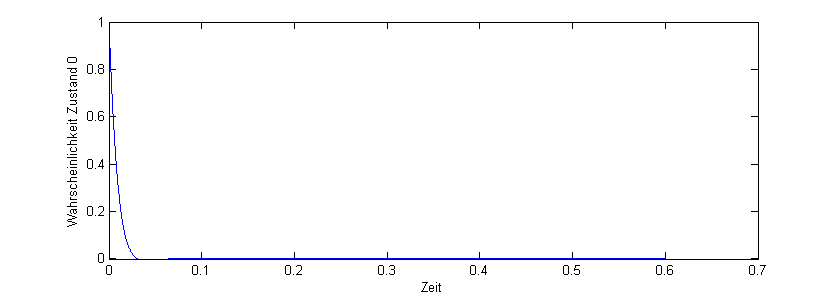
\includegraphics[width=0.7\textwidth]{flash/graphics/StandardZ0.png}
\caption{Abbildung mit mittlerem Potential, dass die Wahrscheinlichkeit 0 ist:
\label{skript:StandardZ0}}
\end{figure}
\begin{figure}
\centering
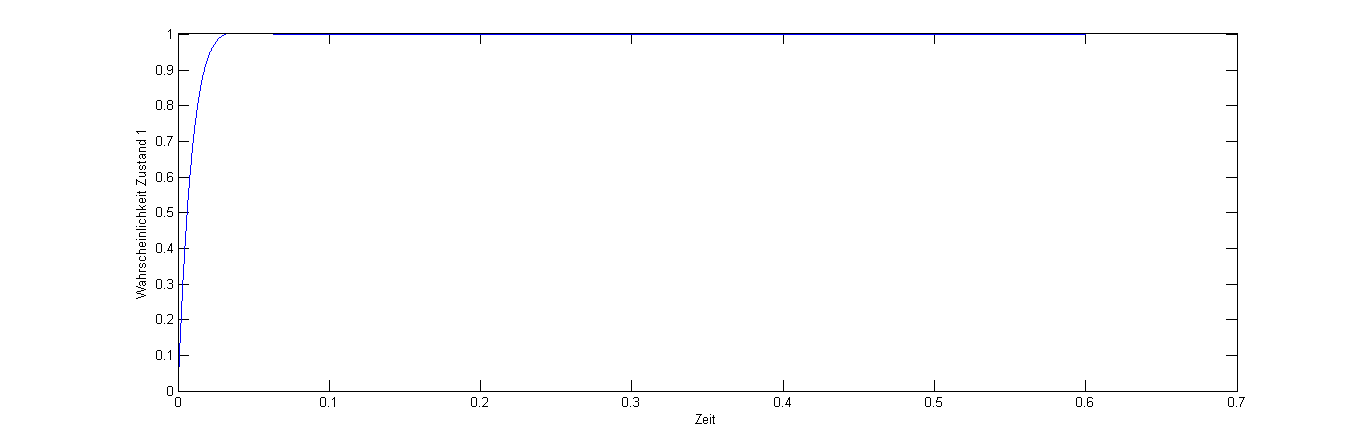
\includegraphics[width=0.7\textwidth]{flash/graphics/StandardZ1.png}
\caption{Abbildung mit mittlerem Potential, dass die Wahrscheinlichkeit 1 ist:
\label{skript:StandardZ1}}
\end{figure}

\begin{figure}
\centering
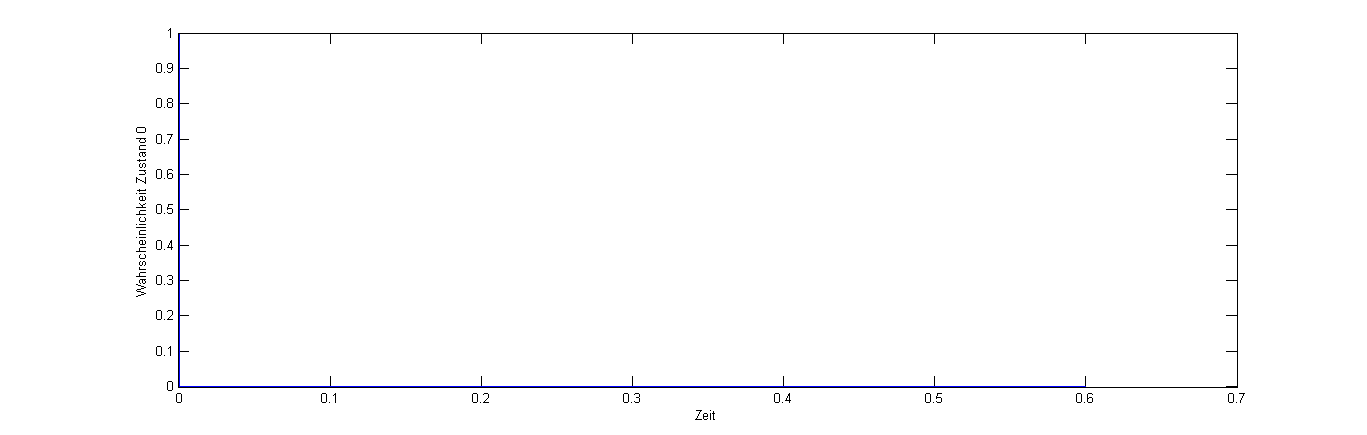
\includegraphics[width=0.7\textwidth]{flash/graphics/PotentialgrossZ0.png}
\caption{Abbildung mit grossem Potential, dass die Wahrscheinlichkeit 0 ist:
\label{skript:PotentialgrossZ0}}
\end{figure}
\begin{figure}
\centering
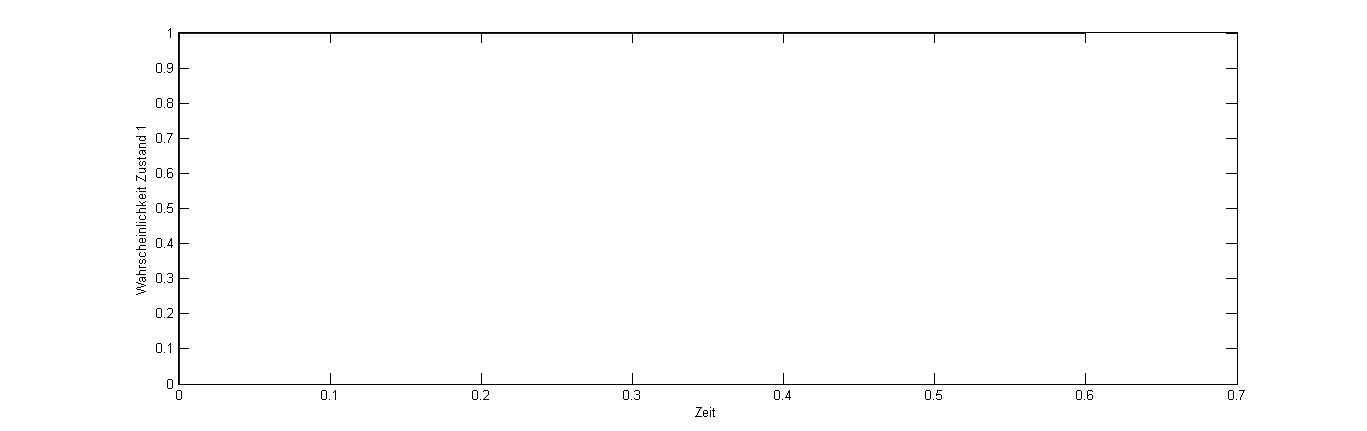
\includegraphics[width=0.7\textwidth]{flash/graphics/PotentialgrossZ1.png}
\caption{Abbildung mit grossem Potential, dass die Wahrscheinlichkeit 1 ist:
\label{skript:PotentialgrossZ1}}
\end{figure}

\begin{figure}
\centering
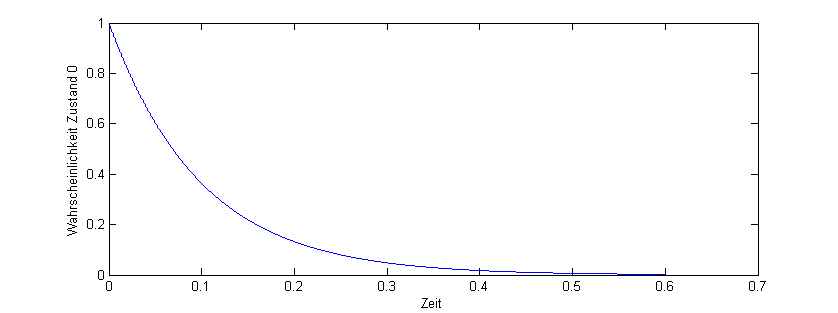
\includegraphics[width=0.7\textwidth]{flash/graphics/PotentialkleinZ0.png}
\caption{Abbildung mit kleinem Potential, dass die Wahrscheinlichkeit 0 ist:
\label{skript:PotentialkleinZ0}}
\end{figure}
\begin{figure}
\centering
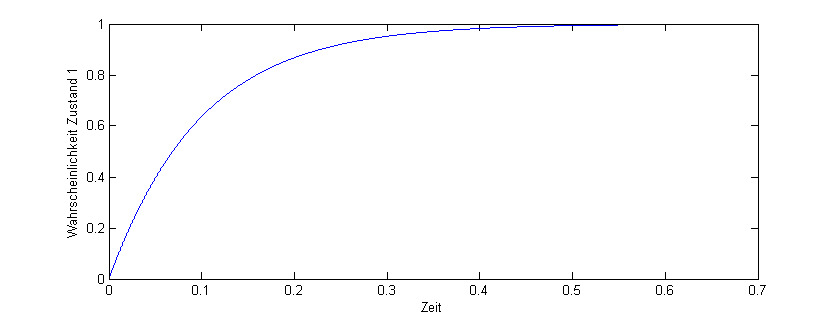
\includegraphics[width=0.7\textwidth]{flash/graphics/PotentialkleinZ1.png}
\caption{Abbildung mit kleinem Potential, dass die Wahrscheinlichkeit 1 ist:
\label{skript:PotentialkleinZ1}}
\end{figure}

\printbibliography[heading=subbibliography]
\end{refsection}

